%% Encoding: ISO8859-1 %%

\section{Grundlagen}

\frame{
\frametitle{Grundlagen}
    \begin{itemize}
        \item token basierte Schaltkreise (Bsp. Petri Netze)
        \item token pass Schaltkreise
        \item nicht polare token pass Brown'sche Schaltkreise
    \end{itemize}
}

%---------------------------------------------------------------------

\frame{
    \frametitle{Token basierte Schaltkreise}
    \begin{itemize}
        \item Signal als Token 
        \item asynchron (kein Takt)
    \end{itemize}

    \begin{figure}   
        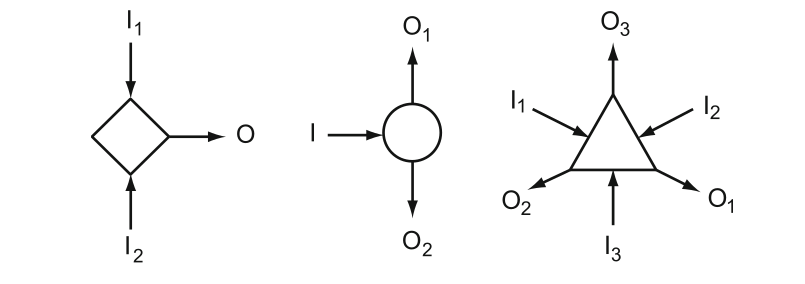
\includegraphics[width=7cm]{bilder/tokenBased.png}
        \caption{Merge, Fork und Tria sind Schaltkreisprimitive}
    \end{figure}
}

%---------------------------------------------------------------------

\frame{
    \frametitle{Token pass Schaltkreise}
    \begin{columns}
        \begin{column}{.5\textwidth}
        \begin{itemize}
            \item Anzahl der Tokens immer gleich
            \item Tokens verlassen Kabel nicht
        \end{itemize}
        \end{column}
        \begin{column}{.5\textwidth} 
            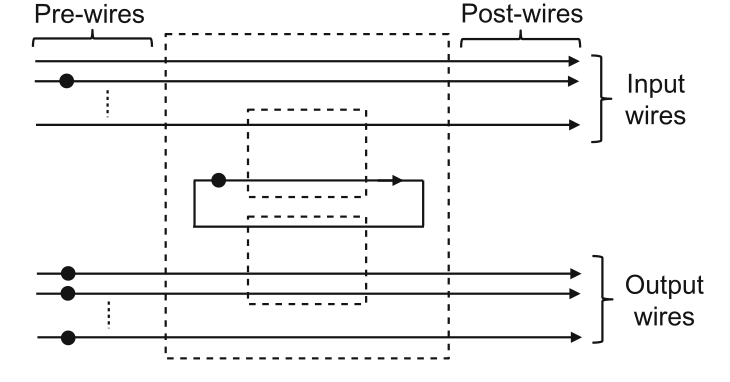
\includegraphics[width=6cm]{bilder/TokenPassScheme.png}
        \end{column}
    \end{columns}
}    

%---------------------------------------------------------------------

\frame{
        \begin{itemize}
            \item Tokens k\"onnen sich frei bewegen 
            \item Verz\"ogerungen beeinflussen nicht Korrektheit der 
                Berechnung
            \item Berechnungsschritte reversibel (Deadlocks)
        \end{itemize}
}

%---------------------------------------------------------------------

%FIXME ueberarbeiten 
\frame{
    \frametitle{T-Element}
    \begin{minipage}{0.45\textwidth}
        \begin{itemize}
            \item \"aquivalent zu Merge 
            \item  
        \end{itemize}
    \end{minipage}\hfill

    \begin{minipage}{0.45\textwidth}
         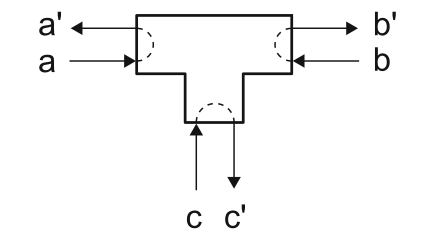
\includegraphics[width=6cm]{bilder/T_Element.png}
    \end{minipage}\hfill

}

%---------------------------------------------------------------------

\frame{
    \frametitle{\"Aquivalenz von token basiert und token pass}
    \centering
    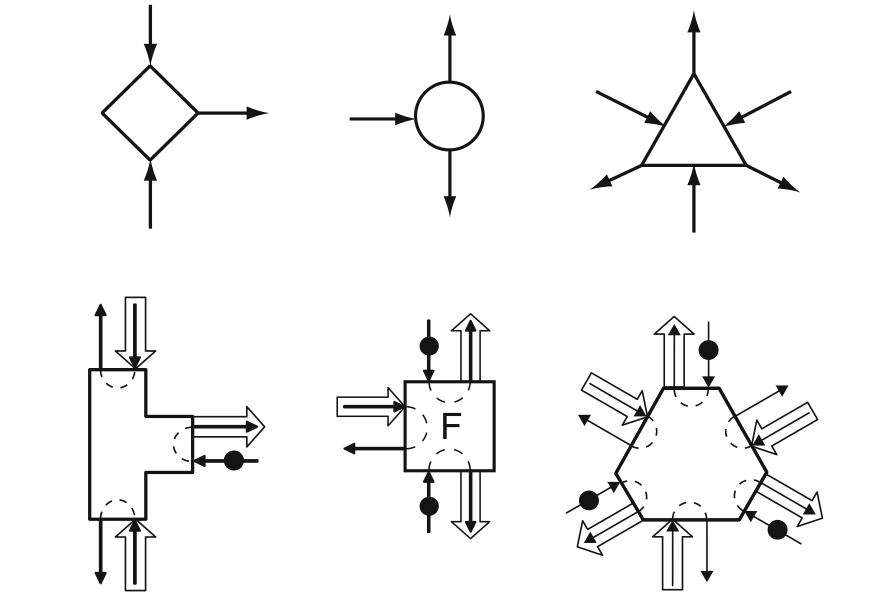
\includegraphics[width=8cm]{bilder/BasedToPass.png}

}

%---------------------------------------------------------------------

\frame{
    \frametitle{\"Aquivalenz von token basiert und token pass}
    \begin{figure}
        \begin{minipage}{0.45\textwidth}
            \centering
            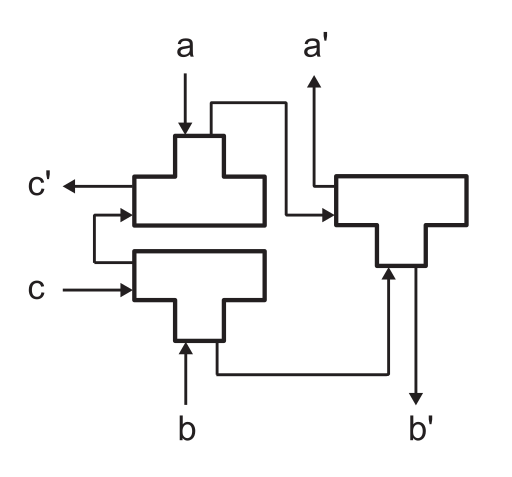
\includegraphics[width=5cm]{bilder/TP_Fork.png}
            \caption{Fork aus T-Elementen}
        \end{minipage}\hfill
        \begin{minipage}{0.45\textwidth}
            \centering
            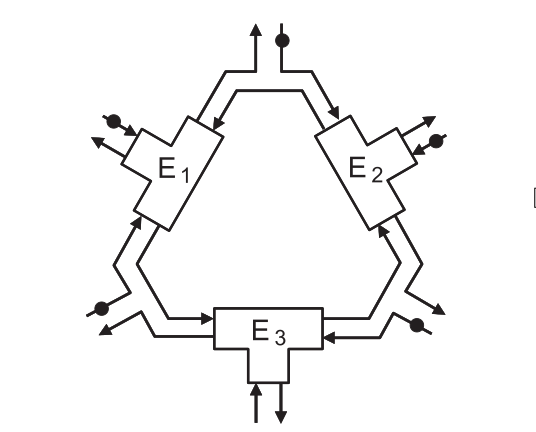
\includegraphics[width=5cm]{bilder/TP_Tria.png}
            \caption{Tria aus T-Elementen}
        \end{minipage}\hfill
    \end{figure}
}

%--------------------------------------------------------------------

\frame{
\frametitle{\"Aquivalenz von token basiert und token pass}
T-Element ist Schaltkreisprimitiv f\"ur brown'sche token pass 
Schaltkreise 
}

%--------------------------------------------------------------------

\frame{
    \frametitle{Nicht polare token pass Schaltkreise}
    \begin{columns}
        \begin{column}{.5\textwidth}
            \begin{itemize}
                \item Tokens haben keinen Bias mehr 
                \item Terminator Kabel 
                \item Bias auf Ein- und Ausgabekabeln sinnvoll
            \end{itemize}
        \end{column}

        \begin{column}{.5\textwidth} 
            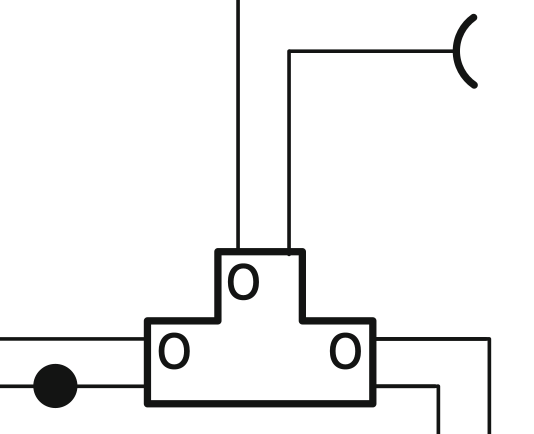
\includegraphics[width=5cm]{bilder/NonPolarTerminator.png}
        \end{column}
    \end{columns}

}

%--------------------------------------------------------------------

\frame{
    \frametitle{Nicht polar token pass Schaltkreise}
T-Element ist Schaltkreisprimitiv f\"ur brown'sche token pass 
Schaltkreise 
}


%--------------------------------------------------------------------
%---------------------------------------------------------------------


\section{1-Bit Speicher}

\frame{
    \frametitle{Nicht polarer 1-Bit Speicher}
    \centering
    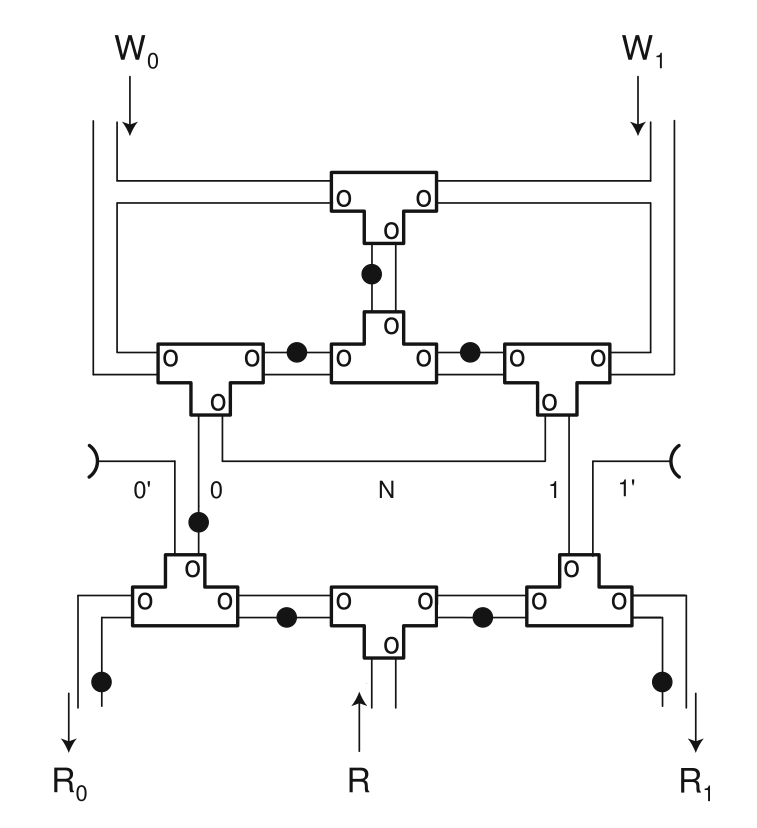
\includegraphics[width=6.5cm]{bilder/NonPolarMemory.png}
}

%---------------------------------------------------------------------

\frame{
    \frametitle{Lesen einer 0}
    \begin{figure}[ht]
        \begin{overlayarea}{7cm}{5cm}
            \includegraphics[width=6.5cm]<1>{bilder/1BitSpeicher/Read_1.png}
            \includegraphics[width=6.5cm]<2>{bilder/1BitSpeicher/Read_2.png}
            \includegraphics[width=6.5cm]<3>{bilder/1BitSpeicher/Read_1.png}
            \includegraphics[width=6.5cm]<4>{bilder/1BitSpeicher/Read_3.png}
            \includegraphics[width=6.5cm]<5>{bilder/1BitSpeicher/Read_4.png}
            \includegraphics[width=6.5cm]<6>{bilder/1BitSpeicher/Read_5.png}
        \end{overlayarea}
    \end{figure}
}

%---------------------------------------------------------------------

\frame{
    \frametitle{Schreiben einer 1}
    \begin{figure}[ht]
        \begin{overlayarea}{7cm}{7cm}
            \includegraphics[width=6cm]<1>{bilder/1BitSpeicher/Write_1.png}
            \includegraphics[width=6cm]<2>{bilder/1BitSpeicher/Write_2.png}
            \includegraphics[width=6cm]<3>{bilder/1BitSpeicher/Write_3.png}
            \includegraphics[width=6cm]<4>{bilder/1BitSpeicher/Write_2.png}
            \includegraphics[width=6cm]<5>{bilder/1BitSpeicher/Write_4.png}
            \includegraphics[width=6cm]<6>{bilder/1BitSpeicher/Write_5.png}
            \includegraphics[width=6cm]<7>{bilder/1BitSpeicher/Write_6.png}
        \end{overlayarea}
    \end{figure}
}

%---------------------------------------------------------------------
%---------------------------------------------------------------------

\section{UND-Gatter} 

\frame{
    \frametitle{UND-Gatter}
    \begin{itemize}
        \item Repr\"asentation von 1 als Token und 0 als Abwesenheit
        \item Repr\"asentation von 1 und 0 als Token 
        \item Ausnutzen des Backtrackings aus Deadlocks
    \end{itemize}
}

%---------------------------------------------------------------------

\frame{
    \frametitle{0 durch kein Token repr\"asentiert}
    \centering
    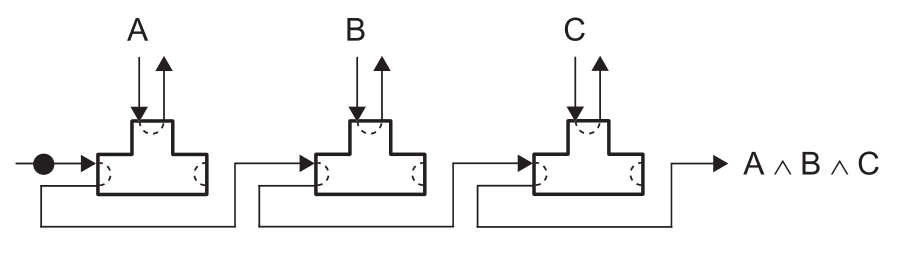
\includegraphics[width=9cm]{bilder/UND_simple.png}
}

%---------------------------------------------------------------------

\frame{
    \frametitle{0 und 1 durch Token repr\"asentiert}
    \centering
    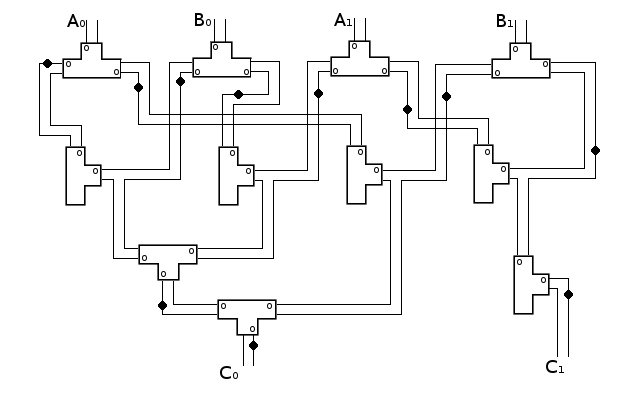
\includegraphics[width=10cm]{bilder/UndGatterOhneRand.png}
}

%---------------------------------------------------------------------

\frame{
    \frametitle{0 und 1 durch Token repr\"asentiert}
    \centering
    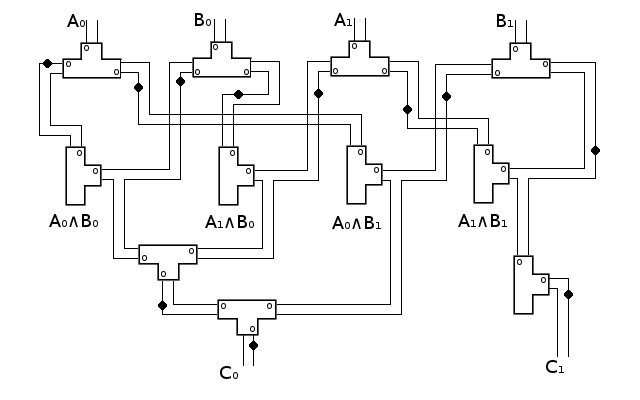
\includegraphics[width=10cm]{bilder/UndGatterOhneRandBeschriftung.png}
}


%---------------------------------------------------------------------
%---------------------------------------------------------------------

\section{Ausblick}

\frame{
    \frametitle{Geschwindigkeit der Berechnung}
}

%---------------------------------------------------------------------

\frame{
    \frametitle{Konkrete Implementierung}
}


%---------------------------------------------------------------------
%---------------------------------------------------------------------


\section{Zusammenfassung} 

\frame{
    \frametitle{Zusammenfassung}
}

